\documentclass[10pt]{article}

\usepackage[T1]{fontenc}
\usepackage[utf8]{inputenc}
\usepackage{lmodern}
\usepackage[margin=2.2cm]{geometry}
\usepackage{amsmath,amssymb}
\usepackage{graphicx}
\usepackage{booktabs}
\usepackage{multirow}
\usepackage{xcolor}
\usepackage{microtype}
\usepackage[hidelinks]{hyperref}

\graphicspath{{../figures/en/}}
% Généré par src/08_paper_assets.py — ne pas modifier à la main.
\newcommand{\resAAAAucA}{0.733}
\newcommand{\resAucAbsAFifty}{0.869}
\newcommand{\resAucAbsATen}{0.735}
\newcommand{\resAucAbsATwentyFive}{0.800}
\newcommand{\resAucAbsBFifty}{0.857}
\newcommand{\resAucAbsBTen}{0.718}
\newcommand{\resAucAbsBTwentyFive}{0.787}
\newcommand{\resAucRelAFifty}{0.878}
\newcommand{\resAucRelATen}{0.749}
\newcommand{\resAucRelATwentyFive}{0.816}
\newcommand{\resAucRelBFifty}{0.871}
\newcommand{\resAucRelBTen}{0.739}
\newcommand{\resAucRelBTwentyFive}{0.808}
\newcommand{\resBBBCost}{0.043}
\newcommand{\resBBBDrift}{+0.19}
\newcommand{\resConcAbs}{0.60}
\newcommand{\resConcGGGAbs}{0.81}
\newcommand{\resConcGGGRel}{0.69}
\newcommand{\resConcRel}{0.81}
\newcommand{\resCostAbs}{0.014}
\newcommand{\resCostGruRel}{0.003}
\newcommand{\resCostRel}{0.008}
\newcommand{\resDriftAbs}{0.135}
\newcommand{\resDriftAbsModelsMax}{0.137}
\newcommand{\resDriftAbsModelsMin}{0.127}
\newcommand{\resDriftRawCommon}{0.135}
\newcommand{\resDriftRecalK}{0.059}
\newcommand{\resDriftRecalT}{0.097}
\newcommand{\resDriftRel}{0.021}
\newcommand{\resDriftRelCommon}{0.043}
\newcommand{\resDriftRelGru}{0.015}
\newcommand{\resDriftRelHgb}{0.051}
\newcommand{\resDriftRelPilot}{0.067}
\newcommand{\resDriftTopQ}{0.058}
\newcommand{\resFoneAbsATwentyFive}{0.653}
\newcommand{\resFoneAbsBTwentyFive}{0.637}
\newcommand{\resFoneRawK}{0.637}
\newcommand{\resFoneRecalK}{0.647}
\newcommand{\resFoneRelATwentyFive}{0.667}
\newcommand{\resFoneRelBTwentyFive}{0.658}
\newcommand{\resFoneRelK}{0.659}
\newcommand{\resFoneTopQK}{0.644}
\newcommand{\resFprGenderAbsA}{$-$0.007}
\newcommand{\resFprGenderAbsACI}{[$-$0.019, +0.005]}
\newcommand{\resFprGenderAbsB}{+0.194}
\newcommand{\resFprGenderAbsBCI}{[+0.180, +0.208]}
\newcommand{\resFprGenderCCCRel}{+0.035}
\newcommand{\resFprGenderCCCRelCI}{[$-$0.014, +0.081]}
\newcommand{\resFprGenderRelB}{+0.015}
\newcommand{\resFprGenderRelBCI}{[+0.003, +0.026]}
\newcommand{\resFprGenderWithinMax}{$-$0.024}
\newcommand{\resFprImdAbsA}{+0.148}
\newcommand{\resFprImdAbsB}{+0.156}
\newcommand{\resFprImdRelB}{+0.116}
\newcommand{\resFprImdRelChange}{$-$0.039}
\newcommand{\resFprImdRelChangeCI}{[$-$0.064, $-$0.017]}
\newcommand{\resGGGAucA}{0.739}
\newcommand{\resGGGClickPctile}{11}
\newcommand{\resGGGDrift}{+0.51}
\newcommand{\resGGGDriftFifty}{+0.51}
\newcommand{\resGGGDriftModelsMax}{+0.53}
\newcommand{\resGGGDriftModelsMin}{+0.47}
\newcommand{\resGGGDriftRecalK}{$-$0.05}
\newcommand{\resGGGDriftRel}{+0.00}
\newcommand{\resGGGDriftRelCommon}{$-$0.14}
\newcommand{\resGGGDriftThirtyThree}{+0.60}
\newcommand{\resGGGFlagA}{44}
\newcommand{\resGGGFlagB}{95}
\newcommand{\resGGGMedClicks}{81}
\newcommand{\resGGGMedScore}{69}
\newcommand{\resGGGNoScore}{47}
\newcommand{\resGGGPrecA}{0.55}
\newcommand{\resGGGPrecB}{0.38}
\newcommand{\resGGGPrecRecalK}{0.55}
\newcommand{\resGGGPrecRecalT}{0.50}
\newcommand{\resGGGRecA}{0.66}
\newcommand{\resGGGRecB}{0.99}
\newcommand{\resGGGRecRecalT}{0.75}
\newcommand{\resGGGRisk}{37}
\newcommand{\resGGGShapDemo}{$-$0.01}
\newcommand{\resGGGShapEngage}{+0.12}
\newcommand{\resGGGShapScores}{+0.19}
\newcommand{\resGGGShapTotal}{+0.30}
\newcommand{\resGGGShapTotalRel}{$-$0.04}
\newcommand{\resGapAbsMax}{0.017}
\newcommand{\resGapAbsMin}{0.012}
\newcommand{\resGapRelMax}{0.010}
\newcommand{\resGapRelMin}{0.007}
\newcommand{\resGapRiskRaw}{0.174}
\newcommand{\resGapRiskRecal}{0.057}
\newcommand{\resGapRiskRefA}{0.059}
\newcommand{\resGapRiskRel}{0.057}
\newcommand{\resGapRiskTopQ}{0.068}
\newcommand{\resGapRiskTopQOracle}{0.003}
\newcommand{\resGoneMax}{28.0}
\newcommand{\resGoneMaxMod}{CCC}
\newcommand{\resGoneMin}{5.4}
\newcommand{\resGoneMinMod}{GGG}
\newcommand{\resGruGainMax}{0.008}
\newcommand{\resGruGainMin}{0.006}
\newcommand{\resNActive}{26,232}
\newcommand{\resNConcImproved}{6}
\newcommand{\resNCorrTests}{69}
\newcommand{\resNEnrol}{32,593}
\newcommand{\resNGenderWithinNeg}{5}
\newcommand{\resNGenderWithinPos}{0}
\newcommand{\resNGenderWithinPosRel}{0}
\newcommand{\resNGoneBeforeStart}{2,678}
\newcommand{\resNImdWithinPos}{5}
\newcommand{\resNModules}{7}
\newcommand{\resNPres}{22}
\newcommand{\resOthersMedClicks}{432}
\newcommand{\resOthersMedScore}{79}
\newcommand{\resPctGone}{19.5}
\newcommand{\resPctLateSub}{4.0}
\newcommand{\resPctWithdrawnGone}{62.5}
\newcommand{\resPlattSdFlag}{0.039}
\newcommand{\resPooledActiveA}{0.815}
\newcommand{\resPooledGap}{0.028}
\newcommand{\resPrecAbsATwentyFive}{0.669}
\newcommand{\resPrecAbsBTwentyFive}{0.618}
\newcommand{\resPrecRawK}{0.619}
\newcommand{\resPrecRawPilot}{0.621}
\newcommand{\resPrecRecalK}{0.624}
\newcommand{\resPrecRecalPilot}{0.615}
\newcommand{\resPrecRelATwentyFive}{0.697}
\newcommand{\resPrecRelBTwentyFive}{0.680}
\newcommand{\resPrecRelK}{0.681}
\newcommand{\resPrecRelPilot}{0.679}
\newcommand{\resPrecTopQK}{0.631}
\newcommand{\resPrecTopQPilot}{0.623}
\newcommand{\resRecAbsATwentyFive}{0.649}
\newcommand{\resRecAbsBTwentyFive}{0.719}
\newcommand{\resRecRelATwentyFive}{0.648}
\newcommand{\resRecRelBTwentyFive}{0.649}
\newcommand{\resRefA}{0.882}
\newcommand{\resRefB}{0.848}
\newcommand{\resRefGap}{0.033}
\newcommand{\resRhoAgeDifficulty}{$-$0.96}
\newcommand{\resRhoAgeDifficultyPres}{$-$0.79}
\newcommand{\resRhoShapDrift}{0.71}
\newcommand{\resRhoWithdrawnDrift}{$-$0.68}
\newcommand{\resRiskActive}{41.4}
\newcommand{\resRiskAll}{52.8}
\newcommand{\resRiskLowClicksGGG}{47}
\newcommand{\resRiskLowClicksOthers}{79}
\newcommand{\resRiskNoScoreGGG}{51}
\newcommand{\resRiskNoScoreOthers}{98}
\newcommand{\resRiskQFive}{33}
\newcommand{\resRiskQOne}{51}
\newcommand{\resSameAggGap}{0.014}
\newcommand{\resSeqGainMax}{0.005}
\newcommand{\resShareFemaleBBB}{88}
\newcommand{\resShareFemaleGGG}{81}
\newcommand{\resStabAbs}{0.81}
\newcommand{\resStabRel}{0.81}
\newcommand{\resTopFiveAbs}{3.3}
\newcommand{\resTopFiveRel}{4.3}
\newcommand{\resWdAucAAbs}{0.651}
\newcommand{\resWdAucARel}{0.675}
\newcommand{\resWdAucBAbs}{0.623}
\newcommand{\resWdAucBRel}{0.662}
\newcommand{\resWdCostAbs}{0.028}
\newcommand{\resWdCostRel}{0.012}
\newcommand{\resWdDriftAbs}{0.054}
\newcommand{\resWdDriftRel}{0.028}
\newcommand{\resWdGGGDriftAbs}{+0.17}
\newcommand{\resWdGGGDriftRel}{+0.03}
\newcommand{\resWdRecBAbs}{0.12}
\newcommand{\resWdRecBRel}{0.10}
\newcommand{\resWdRisk}{13.7}

\newcommand{\cA}{(A)}
\newcommand{\cB}{(B)}
\renewcommand{\thetable}{S\arabic{table}}
\renewcommand{\thefigure}{S\arabic{figure}}
\renewcommand{\thesection}{S\arabic{section}}
\renewcommand{\cite}[1]{}

% Double-blind review: \anonymoustrue hides the authors (same switch as main.tex)
\newif\ifanonymous
\anonymoustrue

\title{Supplementary Material\\[4pt]\large The Ranking Transfers, the Threshold Does Not: Early At-Risk Prediction in Unseen Courses}
\ifanonymous
\author{Anonymous authors}
\else
\author{Doudou Coly, El Hadji Bassirou Tour\'e and El Hadji Mamadou Nguer}
\fi
\date{}

\begin{document}
\maketitle

The numbers in this document are produced by the same script as those of the article (\nolinkurl{src/08_paper_assets.py}), from the outputs of the code repository. Unless stated otherwise, the cut-off is at 25\% of the presentation, only students still enrolled at the cut-off are included, protocol \cB{} is the strict leave-one-module-out, and means are taken over the seven modules.

\section{Remedies per module}
Table~\ref{tab:s-remedies} gives, module by module, the comparison summarized in Table~4 of the article, in the scenario where a random sample of $k=100$ labelled students is available.

\begin{table}[!ht]
\centering
\caption{Remedies per module (25\% cut-off, random sample of $k=100$ labelled students of the target module for Platt and the intercept-only update, mean of 50 draws, standard deviation across draws in parentheses; all rules are evaluated on the remaining students). Top: flag-rate drift $\Delta^{\mathrm{ref}}$ against the absolute-feature model with the module seen. Bottom: precision. Rules as in Table~V of the article.}
\label{tab:s-remedies}
\footnotesize
\begin{tabular}{@{}lcccccc@{}}
\toprule
Module & Raw & Platt & Intercept & Top-$q$ & Top-$q$ (EM) & Relative \\
\midrule
\multicolumn{7}{@{}l}{\emph{Flag-rate drift $\Delta^{\mathrm{ref}}$}} \\
AAA & +0.10 & +0.07 (0.05) & +0.07 (0.05) & +0.07 & $-$0.05 & +0.02 \\
BBB & +0.19 & +0.06 (0.04) & +0.06 (0.04) & +0.05 & +0.37 & +0.03 \\
CCC & $-$0.03 & +0.03 (0.03) & +0.03 (0.03) & $-$0.02 & $-$0.05 & +0.02 \\
DDD & $-$0.05 & +0.02 (0.03) & +0.01 (0.03) & $-$0.04 & $-$0.11 & $-$0.05 \\
EEE & +0.05 & +0.10 (0.04) & +0.08 (0.04) & +0.15 & $-$0.01 & +0.03 \\
FFF & $-$0.03 & +0.07 (0.04) & +0.07 (0.04) & +0.05 & $-$0.16 & +0.01 \\
GGG & +0.51 & $-$0.05 (0.04) & $-$0.03 (0.04) & $-$0.03 & +0.56 & $-$0.14 \\
\midrule
Mean $|\Delta^{\mathrm{ref}}|$ & 0.14 & 0.06 & 0.05 & 0.06 & 0.19 & 0.04 \\
Mean $|$flagged $-$ risk$|$ & 0.17 & 0.06 & 0.06 & 0.07 & 0.22 & 0.06 \\
\midrule
\multicolumn{7}{@{}l}{\emph{Precision}} \\
AAA & 0.38 & 0.39 & 0.38 & 0.38 & 0.42 & 0.45 \\
BBB & 0.54 & 0.60 & 0.60 & 0.61 & 0.47 & 0.67 \\
CCC & 0.78 & 0.74 & 0.74 & 0.77 & 0.69 & 0.72 \\
DDD & 0.79 & 0.75 & 0.76 & 0.78 & 0.81 & 0.81 \\
EEE & 0.70 & 0.66 & 0.67 & 0.60 & 0.74 & 0.72 \\
FFF & 0.76 & 0.69 & 0.70 & 0.70 & 0.87 & 0.76 \\
GGG & 0.38 & 0.55 & 0.54 & 0.56 & 0.37 & 0.64 \\
\midrule
Mean & 0.62 & 0.62 & 0.63 & 0.63 & 0.62 & 0.68 \\
\bottomrule
\end{tabular}
\end{table}


\section{Cohort size}
Table~\ref{tab:s-cohort} shows how the rank model performs when ranks are computed within random sub-cohorts of the target module, over \resNPartitions{} random partitions. With about 50 students or more, ranks are as reliable as when they are computed on the whole presentation. Below 20 students, the gain falls off sharply.

\begin{table}[!ht]
\centering
\caption{Ranks computed in random sub-cohorts of $n$ students of the target module (25\% cut-off, protocol (B), means over modules and over 20 random partitions; interval: 2.5--97.5\% of the module mean across partitions). Shift: absolute change of the share flagged relative to ranks computed on the whole presentation.}
\label{tab:s-cohort}
\footnotesize
\begin{tabular}{@{}lcccccc@{}}
\toprule
$n$ & AUC (B) & 95\% interval & Shift & $|$flagged $-$ risk$|$ & Precision & F1 \\
\midrule
10 & 0.778 & [0.773, 0.781] & 0.042 & 0.082 & 0.677 & 0.617 \\
20 & 0.794 & [0.791, 0.797] & 0.016 & 0.065 & 0.675 & 0.641 \\
50 & 0.802 & [0.800, 0.804] & 0.006 & 0.059 & 0.676 & 0.651 \\
100 & 0.805 & [0.804, 0.806] & 0.004 & 0.058 & 0.678 & 0.655 \\
200 & 0.806 & [0.805, 0.807] & 0.003 & 0.058 & 0.678 & 0.656 \\
whole presentation & 0.808 & --- & 0.000 & 0.057 & 0.680 & 0.658 \\
\bottomrule
\end{tabular}
\end{table}


\section{Average precision}
Average precision, the area under the precision--recall curve, leads to the same conclusions as the AUC (Table~\ref{tab:s-ap}). This also holds for the rarer ``Withdrawn only'' target, whose prevalence is \resWdPrevalence.

\begin{table}[!ht]
\centering
\caption{Average precision (area under the precision--recall curve) at the 25\% cut-off, means over modules.}
\label{tab:s-ap}
\footnotesize
\begin{tabular}{@{}lllccc@{}}
\toprule
Target & Model & Features & Prevalence & AP (A) & AP (B) \\
\midrule
W only & forest & absolute & 0.137 & 0.231 & 0.212 \\
W only & forest & relative & 0.137 & 0.250 & 0.230 \\
W or F & boosting & absolute & 0.387 & 0.748 & 0.728 \\
W or F & boosting & relative & 0.387 & 0.770 & 0.762 \\
W or F & forest & absolute & 0.387 & 0.736 & 0.720 \\
W or F & forest & relative & 0.387 & 0.764 & 0.755 \\
W or F & gru & absolute & 0.387 & 0.735 & 0.729 \\
W or F & gru & relative & 0.387 & 0.765 & 0.763 \\
\bottomrule
\end{tabular}
\end{table}


\section{Intersecting groups}
Table~\ref{tab:s-intersection} gives the false-positive rate of protocol \cB{} when gender is crossed with disability and with the most and least deprived IMD quintiles. With absolute features, disadvantages accumulate: the rate is \resInterFQOneAbs{} for women in the most deprived quintile and \resInterMQFiveAbs{} for men in the least deprived one. With relative features, the remaining gaps follow deprivation rather than gender. Women and men in Q1 have rates of \resInterFQOneRel{} and \resInterMQOneRel, against \resInterMQFiveRel{} for men in Q5.

\begin{table}[!ht]
\centering
\caption{False-positive rates of protocol (B) for intersecting groups (25\% cut-off), with the number of students not at risk in each group and 95\% cluster-bootstrap intervals.}
\label{tab:s-intersection}
\footnotesize
\begin{tabular}{@{}lllrc@{}}
\toprule
Features & Crossing & Group & $n$ (negatives) & FPR [95\% CI] \\
\midrule
absolute & gender x disability & female × no disability & 6,460 & 0.397 [0.386, 0.409] \\
absolute & gender x disability & female × disability & 668 & 0.490 [0.450, 0.527] \\
absolute & gender x disability & male × no disability & 7,716 & 0.205 [0.195, 0.214] \\
absolute & gender x disability & male × disability & 538 & 0.297 [0.258, 0.335] \\
absolute & gender x IMD & female × Q1 & 1,327 & 0.496 [0.471, 0.525] \\
absolute & gender x IMD & female × Q5 & 1,223 & 0.346 [0.320, 0.373] \\
absolute & gender x IMD & male × Q1 & 1,194 & 0.290 [0.265, 0.315] \\
absolute & gender x IMD & male × Q5 & 1,729 & 0.169 [0.152, 0.187] \\
relative & gender x disability & female × no disability & 6,460 & 0.183 [0.174, 0.193] \\
relative & gender x disability & female × disability & 668 & 0.231 [0.200, 0.263] \\
relative & gender x disability & male × no disability & 7,716 & 0.168 [0.159, 0.176] \\
relative & gender x disability & male × disability & 538 & 0.240 [0.207, 0.276] \\
relative & gender x IMD & female × Q1 & 1,327 & 0.260 [0.238, 0.282] \\
relative & gender x IMD & female × Q5 & 1,223 & 0.134 [0.115, 0.155] \\
relative & gender x IMD & male × Q1 & 1,194 & 0.234 [0.208, 0.259] \\
relative & gender x IMD & male × Q5 & 1,729 & 0.129 [0.114, 0.145] \\
\bottomrule
\end{tabular}
\end{table}


\section{Context descriptors associated with transfer}
Table~\ref{tab:corr} lists the associations between context descriptors and the three transfer quantities that remain after Benjamini--Hochberg control. With seven modules, and presentations that are not independent of one another, they should be read as exploratory.

\begin{table}[t]
\centering
\caption{Context descriptors associated with the three transfer axes (Spearman's $\rho$, Benjamini--Hochberg $q < 0.10$ within level, 69 tests in total). Mod.: modules; Pres.: presentations, which are not independent (they share the module-level LOMO model). Difficulty: AUC (A); Rank.\ cost: AUC (A) $-$ AUC (B); Drift: flag-rate drift. Exploratory associations.}
\label{tab:corr}
\footnotesize
\begin{tabular}{@{}llp{3.3cm}rr@{}}
\toprule
Level ($n$) & Axis & Descriptor & $\rho$ & $q$ \\
\midrule
Mod. (7) & Difficulty & Share aged 35+ & $-$0.96 & 0.016 \\
Pres. (22) & Difficulty & Share aged 35+ & $-$0.79 & 0.000 \\
Pres. (22) & Difficulty & VLE activity types & +0.54 & 0.037 \\
Pres. (22) & Difficulty & At-risk rate & +0.49 & 0.060 \\
Pres. (22) & Rank. cost & Assessments due before cut-off & +0.57 & 0.030 \\
Pres. (22) & Rank. cost & First deadline & $-$0.45 & 0.097 \\
Pres. (22) & Drift & Withdrawn share among at-risk & $-$0.68 & 0.008 \\
Pres. (22) & Drift & Share aged 35+ & +0.64 & 0.015 \\
Pres. (22) & Drift & At-risk rate & $-$0.61 & 0.023 \\
Pres. (22) & Drift & Median clicks & $-$0.59 & 0.028 \\
Pres. (22) & Drift & Share without A-level & +0.56 & 0.033 \\
Pres. (22) & Drift & Assessment-structure distance & +0.52 & 0.048 \\
Pres. (22) & Drift & VLE activity types & $-$0.51 & 0.048 \\
Pres. (22) & Drift & Assessments due before cut-off & $-$0.44 & 0.099 \\
\bottomrule
\end{tabular}
\end{table}


\section{Other learners and sequences}
Gradient boosting and a GRU network trained on weekly activity sequences show the same drift with absolute features, and the same correction with relative features (Table~\ref{tab:sequence}, Fig.~\ref{fig:s-sequence}). Temporal information adds little at this early stage. On unseen modules, the GRU does better than the forest by only \resGruGainMin{} to \resGruGainMax{} in AUC, depending on the cut-off.

\begin{table}[t]
\centering
\caption{Model families and temporal information at the 25\% cut-off (students still enrolled; means over modules). Forest and Boosting: aggregated features; Boosting + seq.: aggregated features plus weekly clicks and active days over the complete weeks before the cut-off and trend features; GRU: recurrent network on the weekly sequence plus all static features. Cost: AUC (A) $-$ AUC (B); Drift: mean absolute flag-rate drift; GGG: drift in module GGG.}
\label{tab:sequence}
\footnotesize
\setlength{\tabcolsep}{3pt}
\begin{tabular}{@{}llccccc@{}}
\toprule
Features & Model & AUC (A) & AUC (B) & Cost & Drift & GGG \\
\midrule
\multirow{4}{*}{Absolute} & Forest & 0.800 & 0.787 & +0.014 & 0.135 & +0.51 \\
 & Boosting & 0.805 & 0.787 & +0.018 & 0.137 & +0.53 \\
 & Boosting + seq. & 0.808 & 0.791 & +0.017 & 0.131 & +0.52 \\
 & GRU & 0.799 & 0.792 & +0.007 & 0.127 & +0.47 \\
\midrule
\multirow{4}{*}{Relative} & Forest & 0.816 & 0.808 & +0.008 & 0.021 & +0.00 \\
 & Boosting & 0.818 & 0.811 & +0.007 & 0.051 & +0.01 \\
 & Boosting + seq. & 0.819 & 0.812 & +0.007 & 0.054 & +0.02 \\
 & GRU & 0.817 & 0.815 & +0.003 & 0.015 & +0.00 \\
\bottomrule
\end{tabular}
\end{table}


\begin{figure}[!ht]
\centering
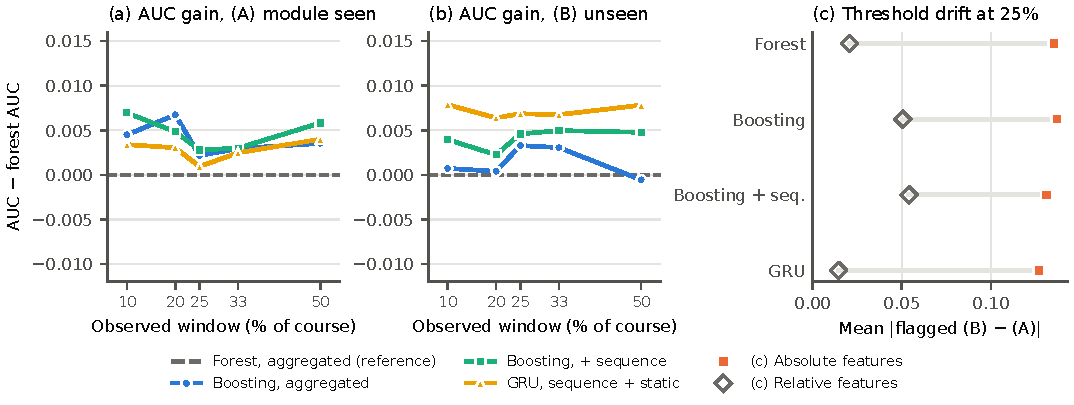
\includegraphics[width=\textwidth]{sequence}
\caption{Sequence models and other learners. (a, b) AUC gain over the random forest on aggregated features (dashed line at zero) with relative features, when the module is seen \cA{} or unseen \cB. (c) Mean absolute flag-rate drift at the 25\% cut-off, with absolute and relative features.}
\label{fig:s-sequence}
\end{figure}

\section{Target definition}
Once the population is restricted to students still enrolled at the cut-off, the ``Withdrawn only'' target amounts to predicting future withdrawal, which is rarer and harder to predict (Table~\ref{tab:target}). The pattern is the same as for the main target. Relative features lower the ranking cost from \resWdCostAbs{} to \resWdCostRel{} and the mean absolute drift from \resWdDriftAbs{} to \resWdDriftRel, and they raise the AUC on unseen modules from \resWdAucBAbs{} to \resWdAucBRel.

\begin{table}[t]
\centering
\caption{Robustness to the target definition (25\% cut-off, students still enrolled; means over modules). W or F: Withdrawn or Fail; W only: Withdrawn only. Abs./rel.: absolute or relative features. Cost: AUC (A) $-$ AUC (B); Drift: mean absolute flag-rate drift.}
\label{tab:target}
\footnotesize
\setlength{\tabcolsep}{3pt}
\begin{tabular}{@{}llcccccc@{}}
\toprule
Target & Feat. & Risk (\%) & AUC (A) & AUC (B) & Cost & Drift & GGG \\
\midrule
W or F & abs. & 38.7 & 0.800 & 0.787 & +0.014 & 0.135 & +0.51 \\
W or F & rel. & 38.7 & 0.816 & 0.808 & +0.008 & 0.021 & +0.00 \\
W only & abs. & 13.7 & 0.651 & 0.623 & +0.028 & 0.054 & +0.17 \\
W only & rel. & 13.7 & 0.675 & 0.662 & +0.012 & 0.028 & +0.03 \\
\bottomrule
\end{tabular}
\end{table}


\section{Further robustness checks}
\paragraph{Threshold.} With absolute features, the mean absolute drift stays between \resThrDriftAbsMin{} and \resThrDriftAbsMax{} for every threshold from 0.3 to 0.7, and the drift of GGG between \resThrGGGAbsMin{} and \resThrGGGAbsMax. With relative features, the mean absolute drift stays between \resThrDriftRelMin{} and \resThrDriftRelMax.

\paragraph{Seeds.} Across \resNSeeds{} seeds, which change both the forest and the assignment of folds, the standard deviation of a module's AUC when it is unseen is at most \resSeedSdAucMax{}, and that of its drift at most \resSeedSdDriftMax.

\paragraph{Standard versus strict hold-out.} If the students who are also enrolled in the held-out module are kept in the training modules, the mean AUC on unseen modules changes by at most \resOverlapMeanDiffMax. In the modules that share many students, removing the shared students changes the AUC of CCC by \resOverlapEffectCCC{} and that of EEE by \resOverlapEffectEEE, whereas removing the same number of randomly chosen enrolments changes it by \resOverlapRandomCCC{} and \resOverlapRandomEEE{} respectively.

\paragraph{Training size.} The training set of \cB{} is \resSizeRatioMin{} to \resSizeRatioMax{} times the size of that of \cA. When the model that has seen the module is trained on exactly as many students as in \cB, the transfer cost is \resSizeCostAbs{} with absolute features and \resSizeCostRel{} with relative features, in line with the main analysis.

\section{Calibration}
Table~\ref{tab:calibration} gives the calibration measures summarized in the article. They compare the transferred model with the model that has seen the module, on the same students, so they measure how much calibration degrades under transfer.

\begin{table*}[t]
\centering
\caption{Calibration of the transferred model at the 25\% cut-off: difference between protocol (B) and protocol (A) on the same students, as the mean absolute difference over modules and for module GGG. Brier score; calibration-in-the-large (intercept of a logistic recalibration with $\mathrm{logit}(\hat{p})$ as offset); mean predicted risk; calibration slope. With balanced class weights the probabilities are not calibrated even in (A), so the transfer effect is the difference (B) $-$ (A).}
\label{tab:calibration}
\footnotesize
\begin{tabular}{@{}lcccccccc@{}}
\toprule
 & \multicolumn{2}{c}{Brier} & \multicolumn{2}{c}{Calibration-in-the-large} & \multicolumn{2}{c}{Mean predicted risk} & \multicolumn{2}{c}{Slope} \\
\cmidrule(lr){2-3}\cmidrule(lr){4-5}\cmidrule(lr){6-7}\cmidrule(l){8-9}
Features & mean $|\Delta|$ & GGG & mean $|\Delta|$ & GGG & mean $|\Delta|$ & GGG & mean $|\Delta|$ & GGG \\
\midrule
Absolute & 0.039 & +0.180 & 0.419 & $-$1.834 & 0.075 & +0.298 & 0.170 & $-$0.321 \\
Relative & 0.006 & +0.004 & 0.079 & $-$0.061 & 0.015 & +0.011 & 0.077 & $-$0.094 \\
\bottomrule
\end{tabular}
\end{table*}


\section{Choice of normalization}
Table~\ref{tab:normalisation} compares percentile ranks with a winsorized z-score and a robust standardization. All three normalize within the cohort, and they give similar results.

\begin{table*}[t]
\centering
\caption{Which cohort normalization? The eight engagement and early-assessment features are normalized within each presentation (weighted forest, 25\% cut-off, LOMO strict, means over modules). $|\Delta^{\mathrm{same}}|$: mean absolute flag-rate drift (B) $-$ (A) of the same variant; $|$flagged $-$ risk$|$: distance between the share flagged in (B) and the observed at-risk rate.}
\label{tab:normalisation}
\footnotesize
\begin{tabular}{@{}lccccccc@{}}
\toprule
Normalization & AUC (A) & AUC (B) & Cost & $|\Delta^{\mathrm{same}}|$ & $|$flagged $-$ risk$|$ & Precision (B) & F1 (B) \\
\midrule
Absolute values & 0.800 & 0.787 & +0.014 & 0.135 & 0.174 & 0.618 & 0.637 \\
Percentile rank & 0.816 & 0.808 & +0.008 & 0.021 & 0.057 & 0.680 & 0.658 \\
z-score (winsorized 1--99\%) & 0.814 & 0.801 & +0.014 & 0.037 & 0.061 & 0.666 & 0.653 \\
Robust (median, IQR) & 0.809 & 0.800 & +0.009 & 0.024 & 0.054 & 0.664 & 0.648 \\
\bottomrule
\end{tabular}
\end{table*}


\end{document}
